\tinysidebar{\debug{exercises/{minimization1/question.tex}}}
  Consider the following two DFAs:
\begin{center}
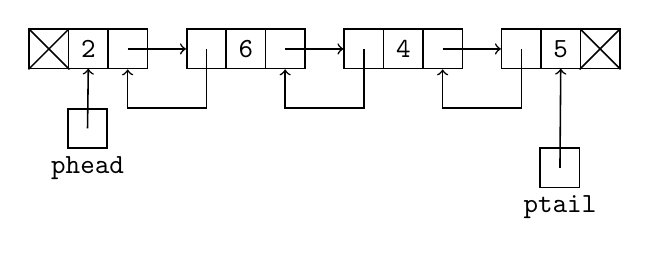
\begin{tikzpicture}

\draw (0.25, 0.25)
  node[draw, line width=0.02cm, , color=black,
       rounded corners=0cm, inner sep=0cm] {

\begin{minipage}[t][0.5cm]{0.5cm}
\mbox{}

\end{minipage}

};\draw (0.25, 0.25) node[color=black] {{\texttt{}}};
\draw (0.75, 0.25)
  node[draw, line width=0.02cm, , color=black,
       rounded corners=0cm, inner sep=0cm] {

\begin{minipage}[t][0.5cm]{0.5cm}
\mbox{}

\end{minipage}

};\draw (0.75, 0.25) node[color=black] {{\texttt{2}}};
\draw (1.25, 0.25)
  node[draw, line width=0.02cm, , color=black,
       rounded corners=0cm, inner sep=0cm] {

\begin{minipage}[t][0.5cm]{0.5cm}
\mbox{}

\end{minipage}

};\draw (1.25, 0.25) node[color=black] {{\texttt{}}};
\draw (2.25, 0.25)
  node[draw, line width=0.02cm, , color=black,
       rounded corners=0cm, inner sep=0cm] {

\begin{minipage}[t][0.5cm]{0.5cm}
\mbox{}

\end{minipage}

};\draw (2.25, 0.25) node[color=black] {{\texttt{}}};
\draw (2.75, 0.25)
  node[draw, line width=0.02cm, , color=black,
       rounded corners=0cm, inner sep=0cm] {

\begin{minipage}[t][0.5cm]{0.5cm}
\mbox{}

\end{minipage}

};\draw (2.75, 0.25) node[color=black] {{\texttt{6}}};
\draw (3.25, 0.25)
  node[draw, line width=0.02cm, , color=black,
       rounded corners=0cm, inner sep=0cm] {

\begin{minipage}[t][0.5cm]{0.5cm}
\mbox{}

\end{minipage}

};\draw (3.25, 0.25) node[color=black] {{\texttt{}}};
\draw (4.25, 0.25)
  node[draw, line width=0.02cm, , color=black,
       rounded corners=0cm, inner sep=0cm] {

\begin{minipage}[t][0.5cm]{0.5cm}
\mbox{}

\end{minipage}

};\draw (4.25, 0.25) node[color=black] {{\texttt{}}};
\draw (4.75, 0.25)
  node[draw, line width=0.02cm, , color=black,
       rounded corners=0cm, inner sep=0cm] {

\begin{minipage}[t][0.5cm]{0.5cm}
\mbox{}

\end{minipage}

};\draw (4.75, 0.25) node[color=black] {{\texttt{4}}};
\draw (5.25, 0.25)
  node[draw, line width=0.02cm, , color=black,
       rounded corners=0cm, inner sep=0cm] {

\begin{minipage}[t][0.5cm]{0.5cm}
\mbox{}

\end{minipage}

};\draw (5.25, 0.25) node[color=black] {{\texttt{}}};
\draw (6.25, 0.25)
  node[draw, line width=0.02cm, , color=black,
       rounded corners=0cm, inner sep=0cm] {

\begin{minipage}[t][0.5cm]{0.5cm}
\mbox{}

\end{minipage}

};\draw (6.25, 0.25) node[color=black] {{\texttt{}}};
\draw (6.75, 0.25)
  node[draw, line width=0.02cm, , color=black,
       rounded corners=0cm, inner sep=0cm] {

\begin{minipage}[t][0.5cm]{0.5cm}
\mbox{}

\end{minipage}

};\draw (6.75, 0.25) node[color=black] {{\texttt{5}}};
\draw (7.25, 0.25)
  node[draw, line width=0.02cm, , color=black,
       rounded corners=0cm, inner sep=0cm] {

\begin{minipage}[t][0.5cm]{0.5cm}
\mbox{}

\end{minipage}

};\draw (7.25, 0.25) node[color=black] {{\texttt{}}};\draw[line width=0.02cm,black,->] (1.25,0.25) to  (1.99,0.25);
\draw[line width=0.02cm,black,->] (3.25,0.25) to  (3.99,0.25);
\draw[line width=0.02cm,black,->] (2.25,0.25) to  (2.25,-0.5) to  (1.25,-0.5) to  (1.25,-0.01);
\draw[line width=0.02cm,black,->] (5.25,0.25) to  (5.99,0.25);
\draw[line width=0.02cm,black,->] (4.25,0.25) to  (4.25,-0.5) to  (3.25,-0.5) to  (3.25,-0.01);
\draw[line width=0.02cm,black,->] (6.25,0.25) to  (6.25,-0.5) to  (5.25,-0.5) to  (5.25,-0.01);
\draw[line width=0.02cm,black] (-0.01,0.51) to  (0.51,-0.01);
\draw[line width=0.02cm,black] (0.51,0.51) to  (-0.01,-0.01);
\draw[line width=0.02cm,black] (6.99,0.51) to  (7.51,-0.01);
\draw[line width=0.02cm,black] (7.51,0.51) to  (6.99,-0.01);

\draw (0.74, -0.76)
  node[draw, line width=0.02cm, , color=black,
       rounded corners=0cm, inner sep=0cm] {

\begin{minipage}[t][0.5cm]{0.5cm}
\mbox{}

\end{minipage}

};\draw (0.74, -0.76) node[color=black] {{\texttt{}}};
\draw (0.74, -1.26)
  node[draw, line width=0.02cm, , color=white,
       rounded corners=0cm, inner sep=0cm] {

\begin{minipage}[t][0.1cm]{0.1cm}
\mbox{}

\end{minipage}

};\draw (0.74, -1.26) node[color=black] {{\texttt{phead}}};\draw[line width=0.02cm,black,->] (0.74,-0.76) to  (0.75,0);

\draw (6.74, -1.26)
  node[draw, line width=0.02cm, , color=black,
       rounded corners=0cm, inner sep=0cm] {

\begin{minipage}[t][0.5cm]{0.5cm}
\mbox{}

\end{minipage}

};\draw (6.74, -1.26) node[color=black] {{\texttt{}}};
\draw (6.74, -1.76)
  node[draw, line width=0.02cm, , color=white,
       rounded corners=0cm, inner sep=0cm] {

\begin{minipage}[t][0.1cm]{0.1cm}
\mbox{}

\end{minipage}

};\draw (6.74, -1.76) node[color=black] {{\texttt{ptail}}};\draw[line width=0.02cm,black,->] (6.74,-1.26) to  (6.75,0);
\end{tikzpicture}

\end{center}


and
\begin{comment}
\begin{center}
\begin{tikzpicture}

\fill[white] (19.0, -0.6) circle (0.3);
\node [line width=0.03cm,black,minimum size=0.57cm,draw,circle] at (19.0,-0.6)(A){};\draw (19.0, -0.6) node[color=black] {\texttt{20}};
\fill[white] (16.0, -1.0) circle (0.3);
\node [line width=0.03cm,black,minimum size=0.57cm,draw,circle] at (16.0,-1.0)(a){};\draw (16.0, -1.0) node[color=black] {\texttt{10}};
\fill[white] (10.0, -2.0) circle (0.3);
\node [line width=0.03cm,black,minimum size=0.57cm,draw,circle] at (10.0,-2.0)(b){};\draw (10.0, -2.0) node[color=black] {\texttt{0}};
\fill[white] (11.0, -4.0) circle (0.3);
\node [line width=0.03cm,black,minimum size=0.57cm,draw,circle] at (11.0,-4.0)(d){};\draw (11.0, -4.0) node[color=black] {\texttt{18}};
\fill[white] (8.0, -3.0) circle (0.3);
\node [line width=0.03cm,black,minimum size=0.57cm,draw,circle] at (8.0,-3.0)(e){};\draw (8.0, -3.0) node[color=black] {\texttt{-2}};
\fill[white] (7.0, -4.0) circle (0.3);
\node [line width=0.03cm,black,minimum size=0.57cm,draw,circle] at (7.0,-4.0)(k){};\draw (7.0, -4.0) node[color=black] {\texttt{-3}};
\fill[white] (9.0, -4.0) circle (0.3);
\node [line width=0.03cm,black,minimum size=0.57cm,draw,circle] at (9.0,-4.0)(l){};\draw (9.0, -4.0) node[color=black] {\texttt{-1}};
\fill[white] (15.0, -4.0) circle (0.3);
\node [line width=0.03cm,black,minimum size=0.57cm,draw,circle] at (15.0,-4.0)(h){};\draw (15.0, -4.0) node[color=black] {\texttt{8}};
\fill[white] (14.0, -5.0) circle (0.3);
\node [line width=0.03cm,black,minimum size=0.57cm,draw,circle] at (14.0,-5.0)(m){};\draw (14.0, -5.0) node[color=black] {\texttt{6}};
\fill[white] (13.0, -3.0) circle (0.3);
\node [line width=0.03cm,black,minimum size=0.57cm,draw,circle] at (13.0,-3.0)(f){};\draw (13.0, -3.0) node[color=black] {\texttt{5}};
\fill[white] (13.0, -6.0) circle (0.3);
\node [line width=0.03cm,black,minimum size=0.57cm,draw,circle] at (13.0,-6.0)(n){};\draw (13.0, -6.0) node[color=black] {\texttt{4}};
\fill[white] (15.0, -6.0) circle (0.3);
\node [line width=0.03cm,black,minimum size=0.57cm,draw,circle] at (15.0,-6.0)(o){};\draw (15.0, -6.0) node[color=black] {\texttt{7}};
\fill[white] (18.0, -2.0) circle (0.3);
\node [line width=0.03cm,black,minimum size=0.57cm,draw,circle] at (18.0,-2.0)(p){};\draw (18.0, -2.0) node[color=black] {\texttt{15}};\draw[line width=0.03cm,black,->,>=triangle 60] (A) to  (a);
\draw[line width=0.03cm,black,->,>=triangle 60] (a) to  (p);
\draw[line width=0.03cm,black,->,>=triangle 60] (a) to  (b);
\draw[line width=0.03cm,black,->,>=triangle 60] (b) to  (e);
\draw[line width=0.03cm,black,->,>=triangle 60] (b) to  (f);
\draw[line width=0.03cm,black,->,>=triangle 60] (f) to  (d);
\draw[line width=0.03cm,black,->,>=triangle 60] (f) to  (h);
\draw[line width=0.03cm,black,->,>=triangle 60] (e) to  (k);
\draw[line width=0.03cm,black,->,>=triangle 60] (e) to  (l);
\draw[line width=0.03cm,black,->,>=triangle 60] (h) to  (m);
\draw[line width=0.03cm,black,->,>=triangle 60] (m) to  (n);
\draw[line width=0.03cm,black,->,>=triangle 60] (m) to  (o);
\end{tikzpicture}

\end{center}


\end{comment}
\begin{center}
\begin{tikzpicture}[>=triangle 60,shorten >=0.5pt,node distance=2cm,auto,initial text=]
\node[state,accepting] (D) at (  3,  0) {$B$};
\node[state,initial] (A) at (  0, -2) {$A$};
\node[state] (B) at (  6, -2) {$C$};
\node[state] (C) at (  3, -4) {$D$};

\path[->]
(A) edge [bend left=0,pos=0.25,above] node {$a$} (B)
(A) edge [bend left=0,pos=0.5,above] node {$b$} (D)
(B) edge [loop above] node {$a$} ()
(B) edge [bend left=10,pos=0.5] node {$b$} (C)
(C) edge [bend left=0,pos=0.5] node {$a$} (A)
(C) edge [bend left=10,pos=0.5,above] node {$b$} (B)
(D) edge [bend left=0,pos=0.5,above] node {$a$} (B)
(D) edge [bend left=0,pos=0.25] node[pos=0.25] {$b$} (C)
;
\end{tikzpicture}
\end{center}
Are they isomorphic?
